\chapter*{Appendices\markboth{Appendices}{}}
\addcontentsline{toc}{chapter}{Appendices}

\clearpage


%-------------------------------------------------------------------- START
\begin{Large}
\textbf{Appendix A} 
\end{Large}
\vspace{3em}

\textbf{Authoring tools in mobile context}

\begin{small}

\em Mobile Author \em \cite{Virvou2005} is a one of the very first mobile authoring tools. This tool contemplates the implementation of only text resources. Moreover, \em Mobile Author \em includes tutoring features to track student’s progress and provides advice adapted to the needs of individual students. This tool was designed assuming that there are two roles, namely, the instructor and the student. In this case, the instructor is the one who authors the lessons and broadcast them to the students in the form of multiple-choice questions, fill-in the blanks and texts, so they can carry out the tasks.

The Remotely Accessible Field Trips (\em RAFT \em) project \cite{Duval2009} is a framework for mobile authoring of learning content in context. The authors discuss the relevancy of contextual metadata for flexible access to learning objects, and, describe approaches for extending current metadata schemas with context metadata. \em RAFT \em makes use of context data to find appropriate use for adaptive learning on demand and personalized learning experiences.

\em StoryKit \em \cite{Bonsignore2013} is a framework for mobile authoring with which children can create original stories, or modify sample stories with their own photos, drawings, and audio. Stories are presented in the form of books. Books can be shared with teachers or colleagues by sending an email (through the mobile app) with the URL of the book in the server, so that the book can be later visualized in a web browser.

Multimedia Presentation Authoring System (\em MPAS \em) \cite{Kim2012} produces multimedia e-learning contents for mobile environment. \em MPAS \em makes possible to create multimedia presentations that integrate diverse media types including images, video, sound, and texts for mobile devices. This proposed system provides an integrated authoring environment that enables authors to produce e-learning contents from media objects and edit or reconstruct existing presentations.

Mobile Authentic Authoring in IMS (\em MAAIMS \em), \cite{Jesse2012} captures authentic learning examples with the mobile device sensors (photo camera, video camera, microphone) which can be supplemented with location aware GPS coordinates and other descriptive metadata following IMS Metadata specifications. \em MAAIMS \em encapsulates these authentic learning examples and employs them as standardized learning objects (IMS Content Packages), and optionally as, standardized learning activities (IMS Learning Designs).

\em Quizzer \em \cite{Giemza2012} enables users to author quizzes in context. Quizzes can be created from scratch or based on existing quizzes. Users can extend or modify quizzes created by others, which will result in separate new quizzes. Optionally, the user can set the location and orientation context for the question. This can either be done manually by pointing on a map and adjusting the orientation value. It can also be done automatically by letting the GPS sensor determine the current location and using the compass for capturing the orientation. In \em Quizzer \em user collaboration is based on exchanging quizzes, scores, ratings and comments.

\em mProducer \em \cite{Wu2006} enables everyday users to perform archiving and editing digital personal experiences from their camera-equipped mobile devices. It also includes sharing features. Nevertheless they do not contemplate remix and recontext.

\em MoVie \em \cite{Multisilta2010} is a social media service that enables users to create video stories using their mobile phones. The staff of a Jazz festival used it for documenting arrangements. The aim was to use the videos for learning how to do things better next year. Supports video sharing and remixing. Moreover, it supports tagging videos by collecting contextual information based on the location of the device.

\end{small}



\clearpage{\pagestyle{empty}\cleardoublepage}
%-------------------------------------------------------------------- END

%-------------------------------------------------------------------- START
\begin{Large}
\textbf{Appendix B} 
\end{Large}
\vspace{3em}

\textbf{Mobile authoring tools classification according to the 10 limitations for universal access to educational resources}

\begin{small}


\begin{figure}[H]
	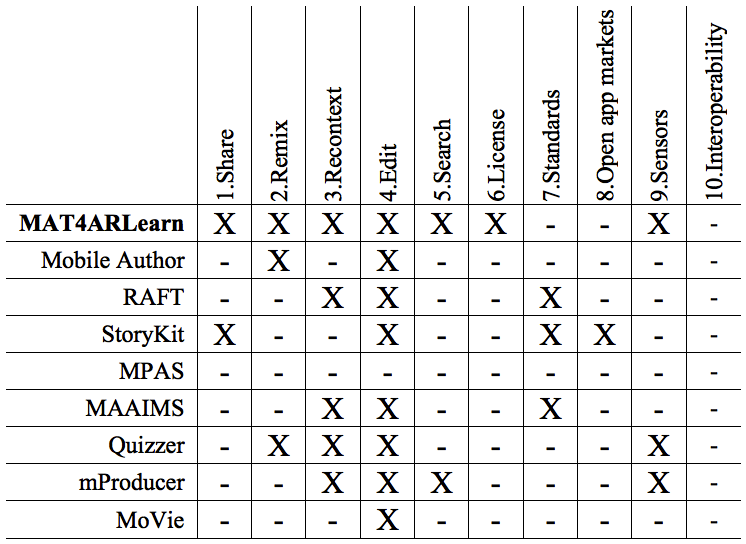
\includegraphics[width=1\linewidth]{img/table3}
	\caption{Mobile authoring tools classification according to features.}
	\label{table3} 
\end{figure}



\end{small}



\clearpage{\pagestyle{empty}\cleardoublepage}
%-------------------------------------------------------------------- END

%-------------------------------------------------------------------- START
\begin{Large}
\textbf{Appendix B} 
\end{Large}
\vspace{3em}

\textbf{Here is the title for appendix B}

\begin{small}

AQUI SE METE LA MOVIDA

\end{small}



\clearpage{\pagestyle{empty}\cleardoublepage}
%-------------------------------------------------------------------- END